\documentclass{csfourzero}
\usepackage{url, natbib, upquote, multicol, caption, subcaption, float, algorithmicx, algpseudocode, enumitem}
\setlength{\bibsep}{0pt plus 0.3ex}
\setitemize[0]{leftmargin=10pt,itemindent=3pt}

\title{The effect of corruption on search engine query correction}
\author{Charlie F.\ Egan}
\date{\today}

\bibliographystyle{plain}
\abstract{Search engines are able to improve query error correction by monitoring user behavior. Rather than relying on traditional spelling correction algorithms alone, the query patterns of users can be built into a more realistic error model. This report investigates the effect of corrupted input on a system's ability to offer accurate corrections. The performance of a number of common search engines is compared and related concepts discussed. It was found that search engines differ significantly in performance and that accuracy is affected by query length.}

\begin{document}
\maketitle

\section{Introduction}
\label{sec:intro}

Search engines that offer corrections to overcome corruption in user queries were the research interest of this project. Corruption is defined as the combined effect of one or more typographical errors. While correction performance is, in cases good, specifics of tools used by search engines to compute corrections are not publicly available. Fundamentally, failed user queries followed by a user's own corrections can build an aggregated list of corrupted queries for an intended result. For longer queries, the probabilities of words in the query context can also be accounted for \cite{noampatent}. Probabilistic edit-distance implementations are also used \cite{howtospellcorrector}.

The project aim was to evaluate the variation in the correction accuracy of a number of common search engines, as well as testing the effect of query length. Correction accuracy is defined as the capability of a search engine to suggest or adopt the intended query, given a corrupted query. This is tested using queries of different lengths for a fixed rate of corruption.

Information about search engine correction accuracy, would be useful for those making mechanical use of search engines. A ranked list of search engines by correction accuracy could also be of interest to those with poor spelling or dexterity caused by conditions such as Dyslexia or Parkinson's disease. More generally, the effect of corrupted string length on the performance of error correction methods for information transfer over an error prone channel is of broader interest.

Sections 2-7 cover spelling correction background as a task within natural language processing, the research questions, the design of the comparison experiments, the results, their discussion and conclusion respectively.

\section{Background and Related Work}
\label{sec:lit}

Computerized spelling correction has been of research interest since 1957 \cite{jameslpeterson1980beginning}. Early approaches offered corrections for strings with typographical errors by calculating edit distance \cite{1992correctiondiscussion}. The edit distance of two strings is the number of edit operations required to transform one string into another \cite{introIR}. In 1966 Levenshtein described a model for such transformations \cite{levenshtein1966binary}. \textit{Levenshtein distance} has been the basis for error models in many implementations since.

However, calculating edit distances between large numbers of strings is computationally expensive \cite{2009adaptivespellchecker}. More recent implementations have used a \textit{Noisy Channel Model}, based on Shannon's \textit{Noisy Channel Theorem}. One such program, named \textit{correct}, detailed in a paper by Kernighan et al. (1990), offered corrections for typographical errors detected by the Unix \textit{spell} program \cite{originalnoisychannel}. The tool generated candidate corrections for a misspelling by applying a single deletion, insertion, transposition or substitution at each position. These candidate corrections are ranked by a combination of their frequency in a larger corpus and the probability of the misspelling given the correction (the noisy channel model). This probability is calculated using \textit{confusion matrices} which store the relative frequencies of different single letter transformations for pairs of letters. This error model was later extended by Brill \& Moore (2000) \cite{betternoisychannel} to represent \textit{string to string} edits for misspellings with multiple errors. Accounting for multiple errors led to a 52\% reduction in the error rate for candidate corrections.

Corruptions of search queries over a noisy channel is comparable to the study of single nucleotide polymorphisms and copy-number variations in Genetics, deep-space telecommunications and wireless video streaming. Error correction is a process beyond spelling.

Search engine query correction poses new challenges and opportunities. 10-15\% of queries contain errors, and short queries make contextual approaches used in word processing of larger documents impractical \cite{webuserpoweredspelling}. Corrections for non-word (typographical) errors are not fully accounted for in dictionaries \cite{webuser3}, for example, \textit{verizon} may be the intended query but would likely be corrected to \textit{version} or \textit{horizon} by a traditional implementation. Real-word or cognitive errors, such as \textit{'an introduction to \textbf{sea} programming'}, are also impossible to model in dictionary implementations.

The first documented approach to make use of user search patterns was that of Brill \& Cucerzan in 2004 \cite{webuserpoweredspelling}. Their implementation compared search engine query logs with a large corpus to gather candidate corrections and used a context-dependent, weighted, edit distance error model to make comparisons. Given that the majority of queries are correct, the transformations can be iteratively applied to arrive at more common (correct) queries. Corrections from the system (the first published approach utilising query logs) aligned 82\% of the time with human annotators with high precision and recall. This approach was improved upon with the inclusion of additional metrics such as page count (for a given query) by Chen et al. (2007) \cite{webuser3}.

A similar approach employed an \textit{Expectation Maximization} algorithm instead of an annotated corpus of corrections \cite{webuser2learningerrormodel}, and while comparable, it did not perform as well as implementations that relied on manually derived information. However, a successful corpus (and language) independent implementation first appeared in 2009, Whitelaw et al. \cite{webuser4google2009}, and was the first system to remove the hand-labeled data requirement. Information about misspellings were inferred from query logs and common queries were used as candidate corrections. The system was fundamentally based on the Noisy Channel Model.

Despite search companies contributing much to the area \cite{webuser3, webuserpoweredspelling, microranker, microphone, webuser4google2009}, comparable information about their implementations was not available. Additionally, the general effect of data length on error correction rates over an error prone channel does not appear to have been studied.

\section{Research question}
\label{sec:rq}

While automated spelling correction is an active topic of research, little is known of the implementations used by search engine companies to calculate corrections. An aim of the project was to superficially investigate these systems and learn how they differ. The effect of query length and the difference in search engine performance were the experimental focus. The research questions for the project were as follows:

\begin{itemize}
  \item{What is the effect of query length on the correction accuracy at a fixed rate of error?}
  \item{Is there a significant difference in correction accuracy between search engines?}
\end{itemize}

\noindent
To address these questions the correction accuracy for a number of search engines was compared. Search engines were tested with corrupted queries of various lengths. Each search engine was tested with the same set of queries and the accuracy of their returned corrections recorded.

The following search engines were tested: \textit{Ask, Baidu, Bing, DuckDuckGo, Google, Sogou, Yahoo, Yandex} and \textit{Youdao}. These non-aggregating search engines all offer corrections for misspellings and also represent the majority of global general search engines \cite{searchenginewiki}. A parallel web scraper was implemented to programmatically run queries and parse results of each search engine for a given query \cite{scraper}. Five instances of this scraper were deployed to disposable environments on the Heroku platform. Requests were then made against each instance to gather results using a local script to aggregate results for each sample.

Due to search engine rate-limiting and time constraints it was infeasible to test large numbers of corrupted queries. Randomly generated seed queries, such as strings of random unrelated words, would not be representative of real world queries. This made the generation of a consistent collection of realistic query phrases challenging without introducing bias. For this experiment, seed terms were selected from the Alexa Top 500 \cite{alexatop500}. The work was built on the assumption that these are a good representation of real user queries. From the 500 domains, only \texttt{.com} variations were used to ensure that each brand was only used once, not for each top-level domain the brand operated. \texttt{.com} brands represent 63\% of the top 500. Seed queries used for generation of the corrupted samples are listed in Appendix 1.

Corruptions were generated from seed queries using a substitution algorithm (Appendix 2). This algorithm, and the possible substitutions for each character, represent the error model of the study. A corruption is applied by selecting a random, unchanged character in the original string and making a substitution with an adjacent key on the keyboard to simulate typographical (non-word) errors. Substitutions are based on the US (UK Macintosh) keyboard and are listed in Appendix 3. Corruptions may be applied a number of times to a seed, however the same index cannot be corrupted more than once. This ensured all corruptions are adjacent keys and that the edit distance was constant within each sample. Substitutions were the only transformations modeled for the study. In a suitably large sample, collisions of corrupted queries and other \textit{valid} queries was assumed to be insignificant.

\section{Experimental Design}
\label{sec:exp}

In response to the research questions, two null hypotheses were set for the study as follows:
\begin{itemize}
  \item{At a constant rate of corruption, accuracy is not significantly affected by the query length in characters. (\textbf{H1})}
  \item{Search engines do not differ significantly in their correction accuracy of corrupted queries. (\textbf{H2})}
\end{itemize}

\noindent
The target population for the study was: all probable user search queries that are the result of one or more typographical errors. Elements at each sample length were based on seed queries, seeds were retained and used to test the corrections returned. Seed queries were selected from website brands of a given length, these were then randomly corrupted at a fixed rate to generate samples. Brands that are either four, eight or twelve characters in length were selected to allow a constant corruption rate of 25\% to be applied. There were no qualifying 16 letter terms. Performance when corrupting a third of the characters was too poor, this made 3,6,9,12,15 an unsuitable set of sample lengths. Seed queries are listed in Appendix 1. There are a greater number of four letter brands, more than three times as many twelve letter terms, though they are distributed among the top domains this source of potential bias was unfortunately unavoidable. All terms on the Alexa list were assumed to have significant search volume at all search engines under test.

At each query length (four, eight and twelve characters), 100 queries were generated from the seeds (Appendix 1) with a constant 25\% corruption rate using the adjacent substitution algorithm (Appendix 2). Substitutions were applied once, twice and three times for four, eight and twelve character seeds respectively - each index was only ever substituted once. For a given sample of corrupted queries, search engine accuracy was defined as the percentage of queries in the sample for which the search engine returns the seed of the corrupted query as a correction on the results page. The seed term is either present or not in the results and it was assumed that, since queries are single words, partial corrections were not possible. The search engine accuracy was the independent variable in all comparisons. Length and search engine were the dependent variables for the first and second questions respectively.

ANOVA and Tukey's HSD statistical tests were used to analyse results. Each query was made using a new session. It was also assumed that search engines operate independently of one and other. The variation of differences from the sample mean accuracy (residuals) were assumed to be normally distributed. Additionally, variance within groups was assumed to be equal.

To test the hypotheses, responses for each of the 100 corrupted queries at each sample length were recorded. The results for all search engines at each length were tested for a group effect. Significant differences in average accuracy between sample lengths was cause to reject the first null hypothesis \textbf{H1}.

To address the second question, using the same set of results, an average score for each search engine was calculated using the results for all lengths. If the differences between these averages were found to be significant, then this would have been cause to reject \textbf{H2}.

\section{Results}
\label{sec:results}

\begin{figure}[H]
  \centering
  \begin{minipage}{.5\textwidth}
    \centering
    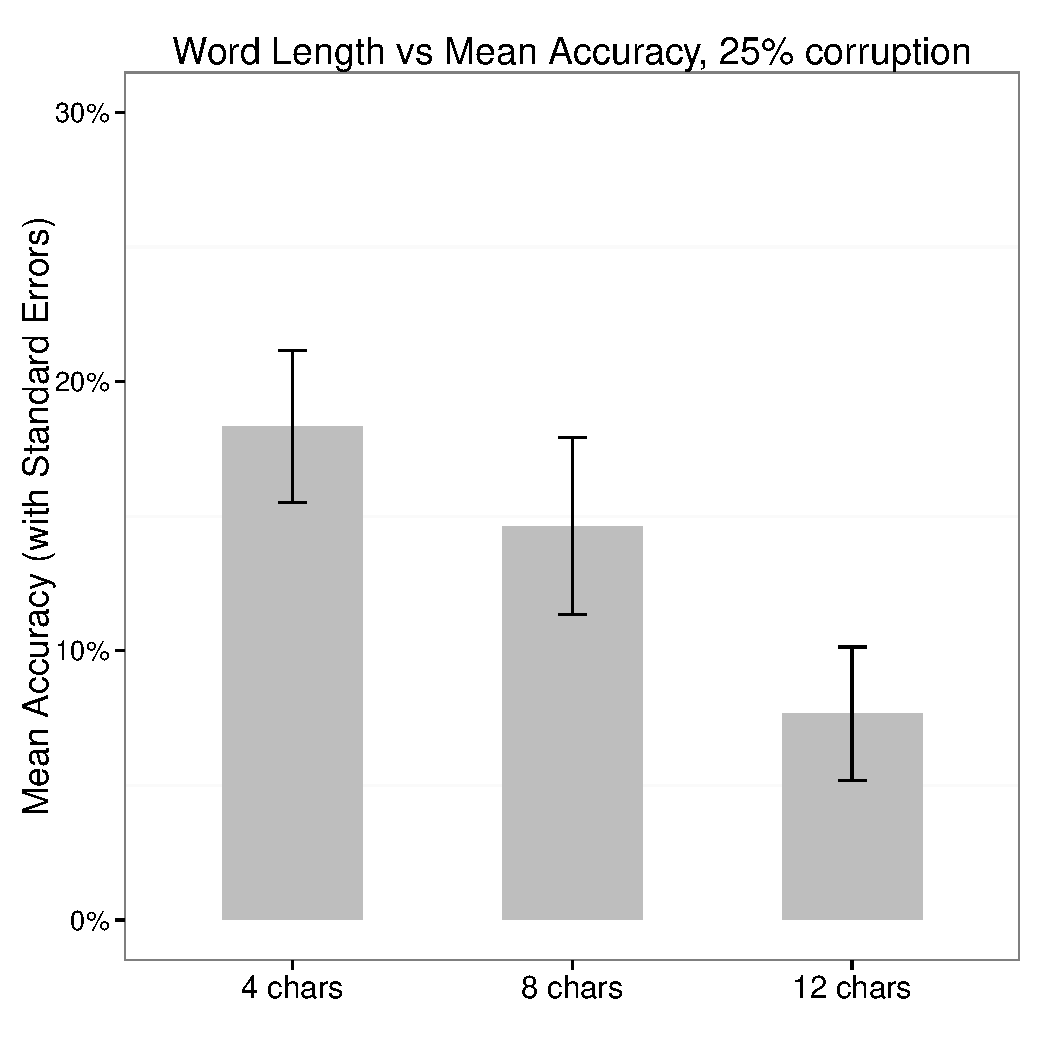
\includegraphics[width=\textwidth]{len_vs_acc}
    \captionof{figure}{Mean search engine accuracy for each query length}
    \label{fig:lengths}
  \end{minipage}%
  \begin{minipage}{.5\textwidth}
    \centering
    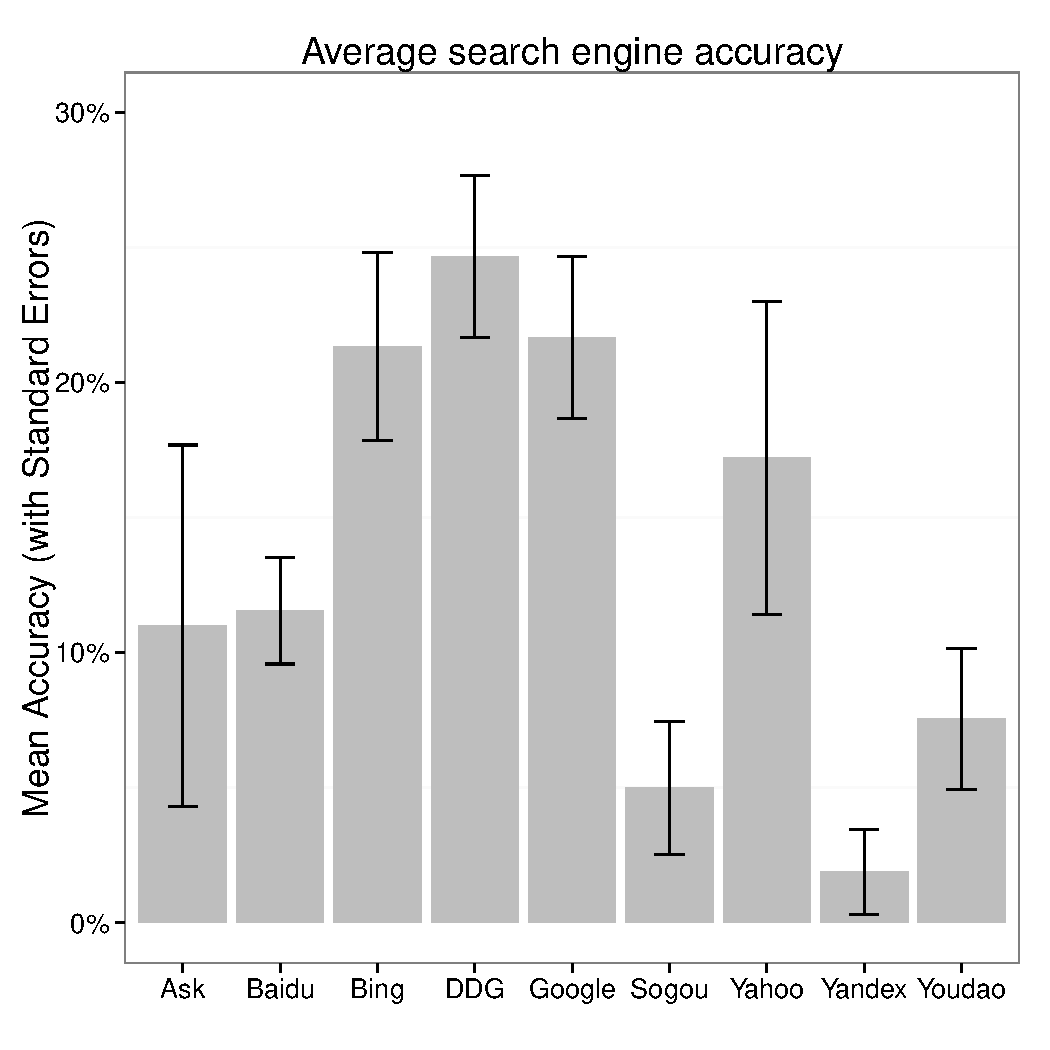
\includegraphics[width=\textwidth]{eng_vs_acc}
    \captionof{figure}{Mean accuracies over all query lengths}
    \label{fig:searchengines}
  \end{minipage}
\end{figure}

Figure~\ref{fig:lengths} shows the average for all nine search engines at each query length. Figure~\ref{fig:searchengines} shows the average accuracy over all query lengths for each search engine. Error bars in both figures represent standard errors in the mean values.

The results suggest that correction accuracy decreases as the query length increases. The effect is most apparent in twelve character queries. While queries four and eight characters in length have more similar accuracy values, they still differ. The results also show a clear difference in search engine correction accuracy performance. Surprisingly, DuckDuckGo returned the most accurate corrections, performing 11\% above average and 23\% above Yandex, the poorest performer. DuckDuckGo is the search engine with the second lowest Alexa rank of those under test. Also of note was the difference between four and eight character lengths for Google - it was the only search engine to perform better on eight character queries.

One way ANOVAs were performed for hypothesis testing. Validation of the ANOVA (and Tukey's HSD) assumptions for the data can be found in Appendix 5.

\subsection{Term length comparison}
Average correction accuracy was calculated using 900 query results across all search engines. An average was calculated for each of the three lengths and plotted in Figure~\ref{fig:lengths}. Using these results, a one-way ANOVA was performed on accuracy and length to make a comparison with \textbf{H1}, that length has no effect on the correction accuracy. The result, $\big((F_{2,24}) = 3.53, p = 0.045\big)$, allows this null hypothesis to be rejected at the 95\% confidence interval as the difference was shown to be significant.

Given that query length has a significant effect on correction accuracy, a Tukey's HSD test was also carried out to closer investigate differences in the means of the three lengths. Only the four vs twelve character comparison gave a result within the 95\% confidence interval $\big(p = 0.038\big)$. Comparisons between adjacent groups were not found to be significant on the data gathered in this project. Both four-eight, and eight-twelve pairwise comparisons resulted in values for $p > 0.2$, $0.64$ and $0.22$ respectively. A larger sample would further refine these values and could reveal a significant difference. The trend was that shorter queries were more accurately corrected with the biggest difference being between the samples for eight and twelve character queries.

\subsection{Search engine comparison}
Using the same data it was possible to also make a comparison between the search engines. Results for all lengths for each search engine were averaged and plotted in Figure~\ref{fig:searchengines}. A one-way ANOVA was performed on accuracy and search engine to examine the difference. This gave a strong result $\big((F_{8,18}) = 4.576, p = 0.0035\big)$ which justifies the rejection of the second null hypothesis \textbf{H2} at the 99\% confidence level.

DuckDuckGo returned the most accurate corrections overall. Bing and Google where close on four and eight characters respectively with eight characters interestingly being the best Google result. Yandex had the poorest correction rate and failed to correct any queries in the twelve character sample, Ask also only returned a single correction for this sample. Please see Appendix 4 for a combined plot comparing the nine search engine average accuracy rates at each length.

\section{Discussion}
\label{sec:discuss}

The results suggest that length impacts correction accuracy, when other variables remain constant. This pattern was consistent across eight of the nine search engines. This suggests shorter queries are better corrected, and more generally, that error correction techniques for corrupted data from an error prone channel are more successful for shorter sequences.

The secondary finding, that search engines differ in correction accuracy, is also of interest. This suggests their query correction implementations differ, though a number of the results are similar. It is also of interest that greater query volume is not required to for best-in-class performance. Google performed worse than DuckDuckGo but handles more than 30 times the number of queries \cite{enginecomparewiki}, unfortunately accurate traffic figures are only available for three of the search engines under test. This would suggest that, despite an apparent trend towards using user activity to train error models \cite{webuserpoweredspelling, webuser3, webuser2learningerrormodel, webuser4google2009}, it is not the only requirement for a high performance implementation. It is also possible that, at a given threshold, additional traffic is no longer beneficial. DuckDuckGo is also the only search engine under test known not to offer personalised results. See Appendix 6 for a plot of search engine Alexa rank against average accuracy.

The length trend is perhaps partially explained by the number of Alexa brands in each category. Four, eight, and twelve characters have counts 35, 28 and \textbf{9} respectively. However, this does not explain the difference in the Google trend. It is possible that the eight letter seed terms are more common queries on Google than other search engines - though this seems unlikely.

The most apparent bias in the study is introduced by the inclusion of both Asian and US search engines. This was done to give sufficient data for each query length - including additional query lengths would have introduced further bias (inconsistent error rate or word count). Seed queries did include Asian brands but the ratio is not comparable to 5:4 US Asia search engines split.

Error generation was also strictly controlled to minimise bias in the length comparison. The algorithm in Appendix 2 is intended to represent realistic typographical errors. Real error models are more representative - but less controlled. Real word errors as well as insertions, deletions and transposition are not covered by this study. A similar comparison based on error types and their positions within a string would be very interesting.

Brand names were selected as seed queries since they are likely to be consistently well ranked. However, they do not allow for a wide range in query lengths without introducing potential bias from word count differences. A repeat study that used a wider range of query lengths would make for a good comparison. Wikipedia article titles were considered for this study.

The experiment design was focused on the first question. A more detailed, search engine centric, comparison would include a wider range of query types and errors as detailed above. This study was based on ``Did you mean" prompts, another more realistic metric would be checking the relevance of the first result for a corrupted query.

\section{Conclusion}
\label{sec:conc}

This study investigated the effect of query length on error correction accuracy by testing responses for queries with non-word errors from a number of search engines. This was done to better understand error correction, and more specifically, the effect of query length. The results suggest that increasing length has a negative impact on correction accuracy, even when corruption is constant. They also show a clear, and in cases unexpected, difference in the accuracy between search engines, e.g. Google's four and Yahoo's twelve character performance. These results highlight areas for further error correction development.

\raggedbottom
\pagebreak
\bibliography{myrefs}

\pagebreak
\raggedbottom
\section{Appendix 1: Seed Terms}
\textbf{Four Letter Seeds}
\textit{\{Ebay, Bing, Imdb, Etsy, Yelp, Cnet, Vice, Ikea, 9gag, Hulu, Dell, Citi, Asos, Java\}}

\noindent
\textbf{Eight Letter Seeds}
\textit{\{Linkedin, Blogspot, Flipkart, Outbrain, Buzzfeed, Whatsapp, Softonic, Usatoday, Mashable, Engadget, Gsmarena, Evernote, Theverge\}}

\noindent
\textbf{Twelve Letter Seeds}
\textit{{Spaceshipads, Secureserver, Shutterstock, Espncricinfo, Steampowered, Mercadolivre, Extratorrent, Liveinternet, Infusionsoft, Surveymonkey}}

\pagebreak
\raggedbottom
\section{Appendix 2: Corruption Algorithm}
  \begin{algorithmic}
    \Function{corruptString}{$string$, $count$}
        \State $string \gets downcase(string)$
        \State $indexes \gets$ $\{ x \in \mathbb{Z} \ \vert \ 1 \leq x \leq length(string) \}$
        \State $indexes \gets$ $randomOrder(indexes)$
        \Repeat
        \State $indexToCorrupt \gets pop(indexes)$
        \State $characterToCorrupt \gets string[indexToCorrupt]$
        \State $replacementCharacters \gets keyboardSubstitutionsForCharacter(characterToCorrupt)$
        \State $string[indexToCorrupt] \gets randomElement(replacementCharacters)$
        \State $count \gets count - 1$
        \Until{count is 0}
        \State \Return $string$
    \EndFunction
  \end{algorithmic}

\pagebreak
\raggedbottom
\section{Appendix 3: Letter Substitutions}
\begin{multicols}{2}
  \begin{verbatim}
  a : {q w s z `}
  b : {v g h n}
  c : {x d f v}
  d : {s e r f c x}
  e : {w 3 4 r d s}
  f : {d r t g v c}
  g : {f t y h b v}
  h : {g y u j n b}
  i : {u 8 9 o k j}
  j : {h u i k m n}
  k : {j i o l , m}
  l : {k o p ; . ,}
  m : {n j k ,}
  n : {b h j m}
  o : {i 9 0 p l k}
  p : {o 0 - [ ; l}
  q : {1 2 w a}
  r : {e 4 5 t f d}
  s : {a w e d x z}
  t : {r 5 6 y g f}
  u : {y 7 8 i j h}
  v : {c f g b}
  w : {q 2 3 e s a}
  x : {z s d c}
  y : {t 6 7 u h g}
  z : {` a s x}
  . : {, l ; /}
  ! : {@ 2 1 q §}
  0 : {- p o 9}
  1 : {§ q 2}
  2 : {1 q w 3}
  3 : {2 w e 4}
  4 : {3 e r 5}
  5 : {4 r t 6}
  6 : {5 t y 7}
  7 : {6 y u 8}
  8 : {7 u i 9}
  9 : {8 i o 0}
  - : {0 p [ =}
  \end{verbatim}
\end{multicols}


\pagebreak
\section{Appendix 4: Detailed Search Engine Plot}
\begin{figure}[H]
  \centerline{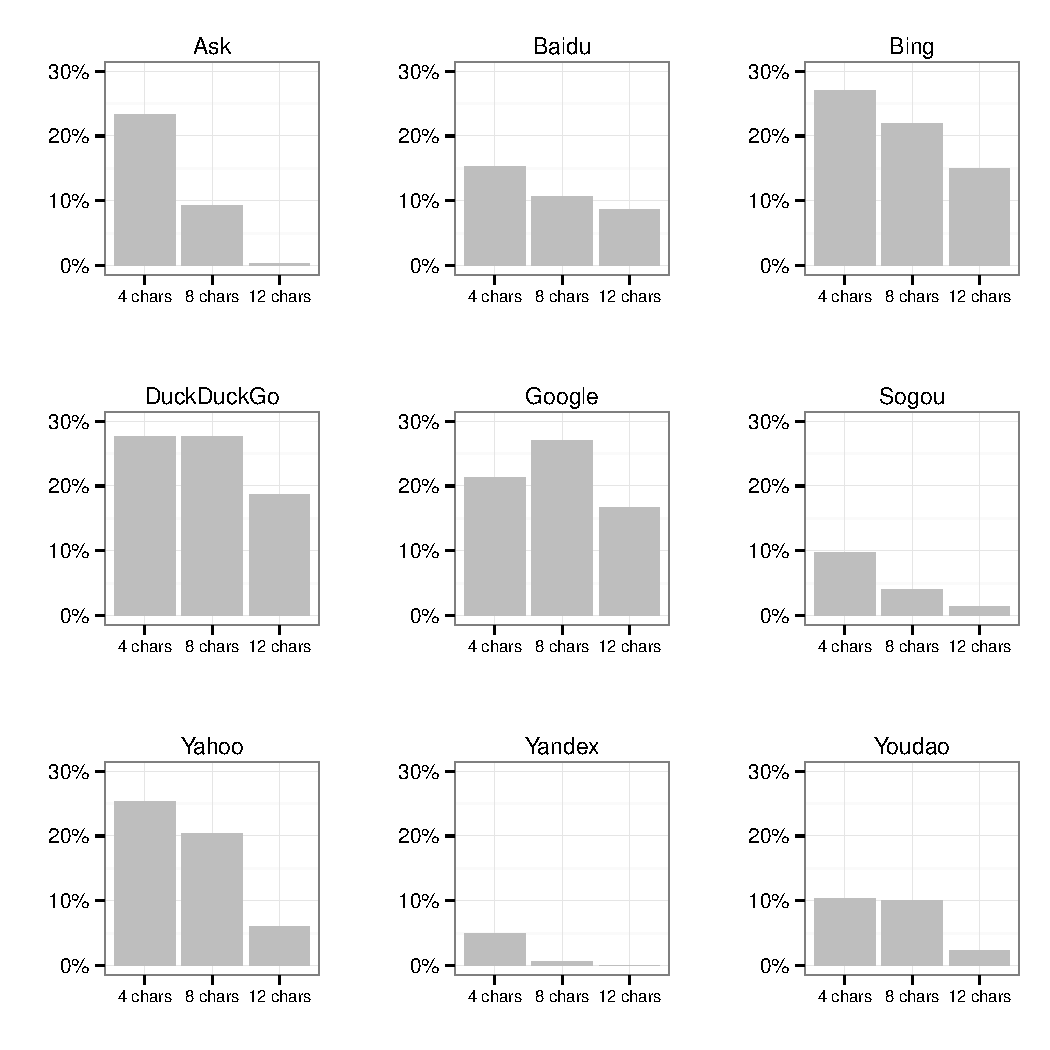
\includegraphics[width=\textwidth]{eng_vs_acc_9_way}}
  \caption{Accuracies for each length of each search engine compared}\label{fig:9searchengines}
\end{figure}

\pagebreak
\section{Appendix 5: ANOVA Assumption Validation}
\subsection{Independence of Observations}
Search engines are assumed to operate independently. Each query is made programmatically using a fresh session.

\subsection{Equality of Variances}
Bartlett K-squared results do not give cause to reject the test's null hypothesis, that the variances are equal. Results are as follows:
\begin{itemize}
  \item{\textbf{Length:} $\chi^2 = 0.63, p = 0.73 $}
  \item{\textbf{Search Engine:} $\chi^2 = 6.23, p = 0.62 $}
\end{itemize}

\subsection{Normality}
\begin{figure}[H]
  \centerline{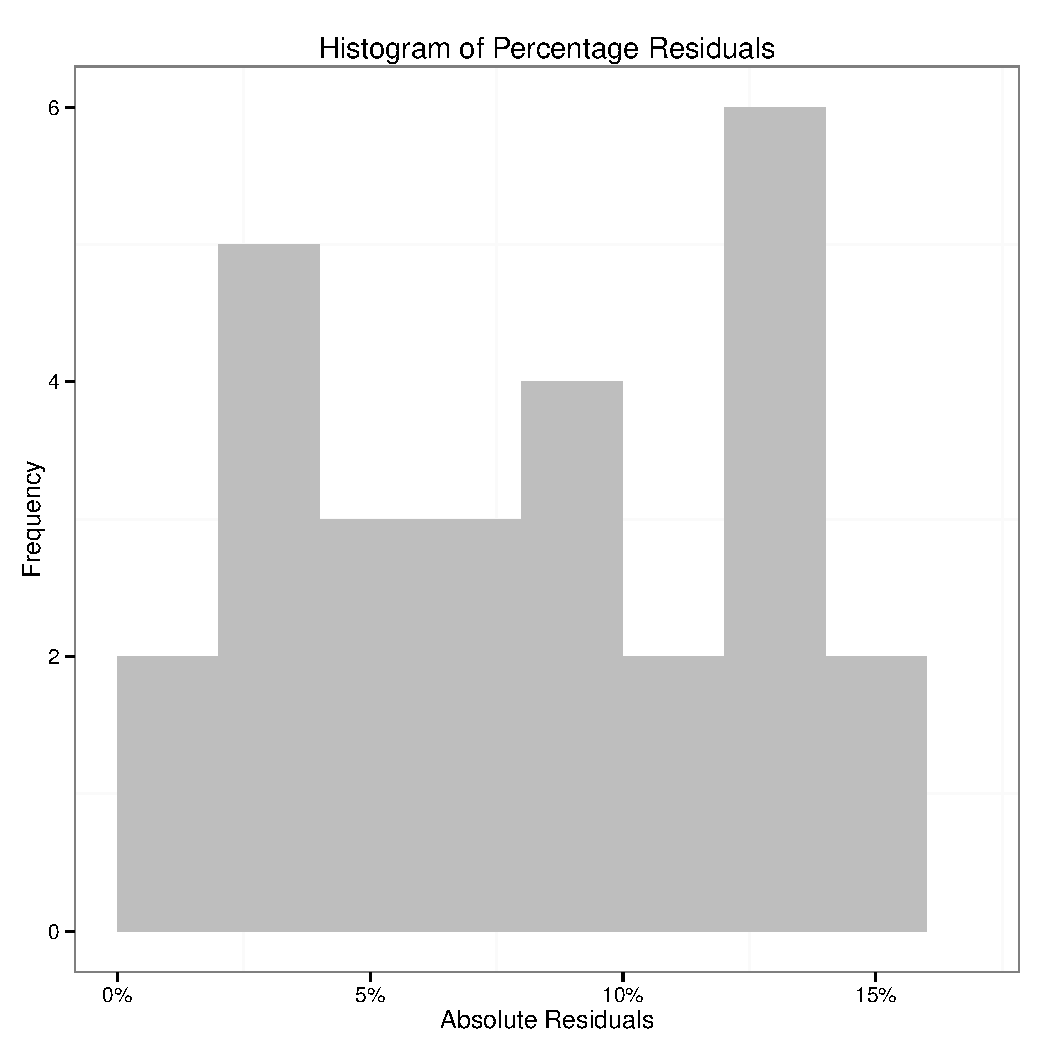
\includegraphics[width=0.7\textwidth]{residual_histogram}}
  \caption{Distribution of accuracy residuals of for lengths and search engines}\label{fig:9searchengines}
\end{figure}

\pagebreak
\section{Appendix 6: Alexa Rank Accuracy Plot}
\begin{figure}[H]
  \centerline{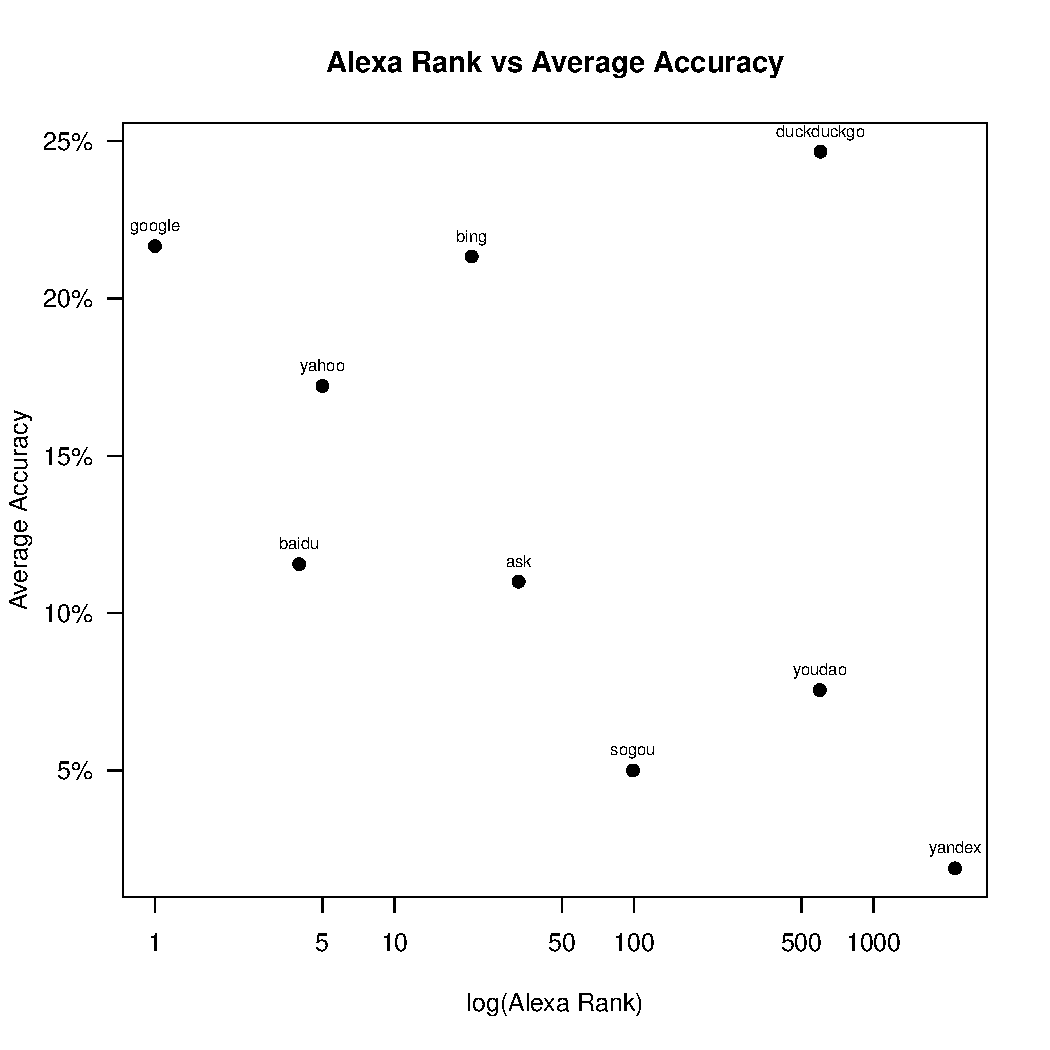
\includegraphics[width=0.7\textwidth]{rank_scatter}}
  \caption{Alexa rank vs average accuracy for each search engine, showing DuckDuckGo as a clear outlier}\label{fig:9searchengines}
\end{figure}

\end{document}
